\subsection{Structure}

During this development phase, we focused on building each physical component of the robot's structure based on the technical drawings and models defined in the previous stage. The entire chassis was built of wood using standard tools available in Bovisa's \textit{Prototipi} lab. This choice of material allowed for fast prototyping, easy modifications, and rigid support for the movement module.

\subsubsection{Base panel}
This large dodecagonal panel serves as the foundation for the robot. It supports the motors, the battery, and the lower part of the vertical columns. We cut it from an MDF panel (220 x 152 cm, 3mm) with precision to match the dimensions in the technical drawing, ensuring symmetry and enough surface area for wheel spacing and internal wiring. It serves to mount the electronics and vertical panels and helps complete the structural frame.

\begin{figure}[H]
    \centering
    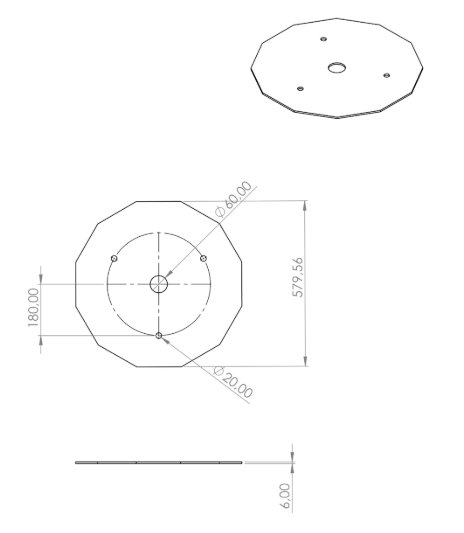
\includegraphics[width=0.6\linewidth]{../ReportMovementModule/images/Aspose.Words.728084da-df58-4b9d-a372-f65cffbdb23d.018.jpeg}
    \caption{Base Panel}
\end{figure}

\subsubsection{Upper platform}
This smaller dodecagonal plate forms the top of the movement module. We constructed it to match the base's outer shape but at a smaller scale. It serves to mount the other modules and helps complete the structural frame.

\begin{figure}[H]
    \centering
    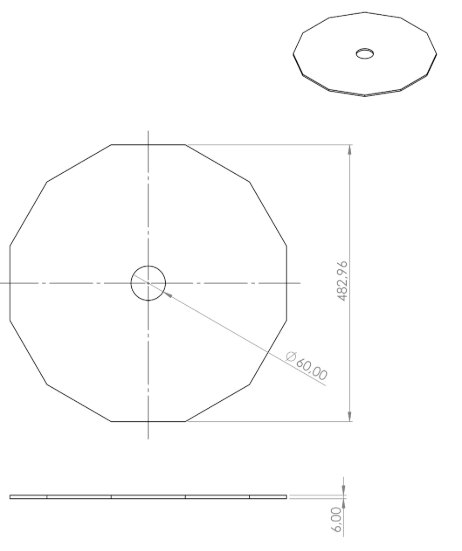
\includegraphics[width=0.6\linewidth]{../ReportMovementModule/images/Aspose.Words.728084da-df58-4b9d-a372-f65cffbdb23d.019.jpeg}
    \caption{Upper Platform}
\end{figure}

\subsubsection{Lower platform}
This element was originally designed as a lower platform, located below the main base. Its purpose was to hold some of the electronic components, freeing up space on the main base. However, during the assembly and testing phase, we encountered a practical issue: this platform reduced the vertical clearance between the wheels and the ground, interfering with proper contact and compromising movement. In sight of this we decided to remove this platform and relocate its electronic components in the bottom face of the base panel.

\begin{figure}[H]
    \centering
    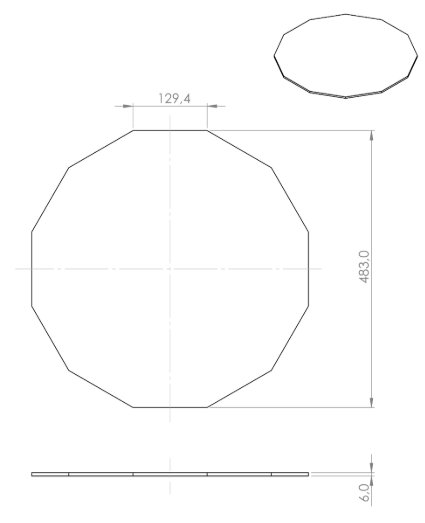
\includegraphics[width=0.6\linewidth]{../ReportMovementModule/images/Aspose.Words.728084da-df58-4b9d-a372-f65cffbdb23d.020.jpeg}
    \caption{Lower Platform (Later Removed)}
\end{figure}

\subsubsection{Columns}
Three vertical wooden rods were cut and sanded to precise height to connect the base and the top plate. They ensure the structure is rigid and that both plates remain parallel.

\begin{figure}[H]
    \centering
    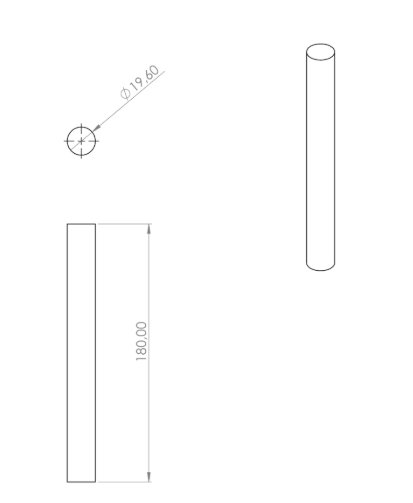
\includegraphics[width=0.6\linewidth]{../ReportMovementModule/images/Aspose.Words.728084da-df58-4b9d-a372-f65cffbdb23d.021.jpeg}
    \caption{Vertical Column}
\end{figure}

\subsubsection{Columns supports}
These wooden components serve as the \textbf{connection points between structural levels}. Three of them are placed between \textbf{the lower platform and the base panel}, acting as a solid foundation and providing vertical spacing. The other three are positioned \textbf{between the top ends of the columns and the upper platform}, ensuring a stable connection. There are in total six units of these types of pieces, which help to distribute weight and keep the vertical supports firmly aligned, contributing significantly to the overall rigidity and symmetry of the structure.

\begin{figure}[H]
    \centering
    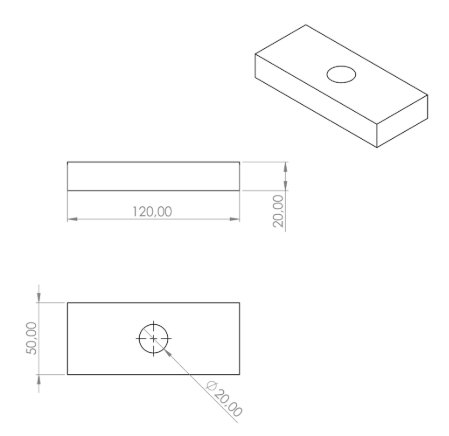
\includegraphics[width=0.6\linewidth]{../ReportMovementModule/images/Aspose.Words.728084da-df58-4b9d-a372-f65cffbdb23d.022.jpeg}
    \caption{Column Supports}
\end{figure}

Each part was cut, assembled, and adjusted manually, allowing us to iteratively test fit and stability during the process. The built structure was robust enough to support the entire electronic system and the external aesthetic modules, while remaining accessible for maintenance and future upgrades.

\begin{figure}[H]
    \centering
    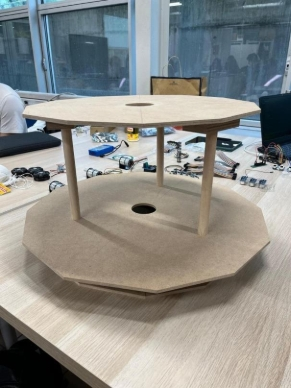
\includegraphics[width=0.6\linewidth]{../ReportMovementModule/images/Aspose.Words.728084da-df58-4b9d-a372-f65cffbdb23d.023.jpeg}
    \caption{Assembled Structure}
\end{figure}

However, during testing, we found that this additional level \textbf{reduced the clearance between the omnidirectional wheels and the ground}, which significantly affected the robot's ability to move.

To resolve this, we decided to \textbf{remove the lower platform entirely}. As an alternative, we reorganized the layout of the components. The \textbf{electronic modules that were originally intended to be mounted on the removed platform were relocated} to the \textbf{base panel}. In the bottom face of the base panels three additional pieces like the ones that can be seen in the image were assembled to have more space for relocating the electronic modules. This change improved ground contact for the wheels and simplified the structural layout, while still maintaining proper distribution of the components across the chassis.

\begin{figure}[H]
    \centering
    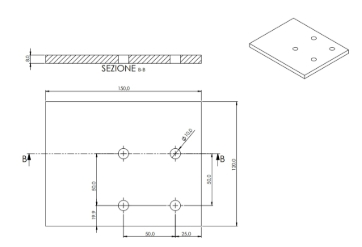
\includegraphics[width=0.6\linewidth]{../ReportMovementModule/images/Aspose.Words.728084da-df58-4b9d-a372-f65cffbdb23d.024.jpeg}
    \caption{Modified Structure}
\end{figure}

\begin{figure}[H]
    \centering
    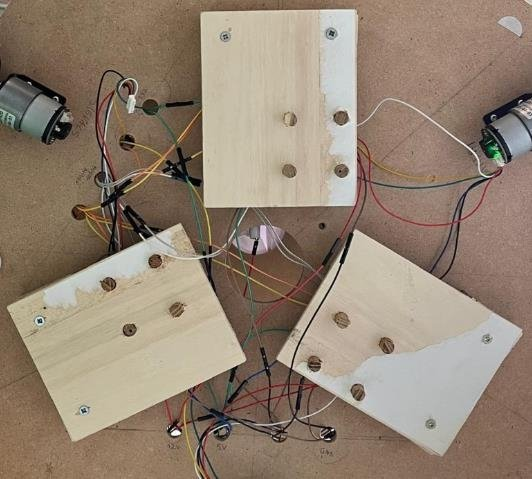
\includegraphics[width=0.6\linewidth]{../ReportMovementModule/images/Aspose.Words.728084da-df58-4b9d-a372-f65cffbdb23d.025.jpeg}
    \caption{Final Structure Configuration}
\end{figure}
